
%(BEGIN_QUESTION)
% Copyright 2014, Tony R. Kuphaldt, released under the Creative Commons Attribution License (v 1.0)
% This means you may do almost anything with this work of mine, so long as you give me proper credit

Use Kirchhoff's Voltage Law to calculate the magnitude and polarity of the voltage across resistors $R_2$ and $R_4$ in this resistor network:

$$\includegraphics[width=15.5cm]{i01156x01.eps}$$

\underbar{file i01156}
%(END_QUESTION)





%(BEGIN_ANSWER)

$$\includegraphics[width=15.5cm]{i01156x02.eps}$$

%(END_ANSWER)





%(BEGIN_NOTES)

In your discussion, be sure to explore more than one ``loop'' when using KVL.  Not only does this demonstrate the arbitrary nature of your loop choice, but it also serves as a double-check for your work!

It is not necessary to know anything about series-parallel or even parallel circuits in order to solve for $R_2$'s or $R_4$'s voltage -- all one needs to know is how to use Kirchhoff's Voltage Law.

%INDEX% Electronics review: series-parallel circuits

%(END_NOTES)


